\documentclass[fontsize=12pt,a4paper]{scrreprt}

\usepackage[utf8]{inputenc}
\usepackage[margin=1in,heightrounded]{geometry}
\usepackage{hyperref}
\usepackage{graphicx}
\usepackage{lipsum}
\usepackage[T1]{fontenc} % prevents < in text mode turning into
\usepackage{textcomp}    % ?', etc
\usepackage[osf]{mathpazo} % Palatino font
\usepackage[scaled=.9]{helvet} % nice san serif fonts
\usepackage{microtype} % micro-typographical extensions
\usepackage[british]{babel} % British hyphenation patterns, etc.
\usepackage{paralist}
\usepackage{tabularx}
\usepackage{booktabs}
\usepackage[section]{placeins}

\renewcommand*{\chapterheadstartvskip}{\vspace*{-\topskip}}
\setlength{\parskip}{.5em}

\pagestyle{headings}

\author{Y0070944}
\title{IAPT Longboxes Design Document}

\begin{document}

\maketitle
\setcounter{page}{1}

%-------------------------------------------------------------------------------
\chapter{Data Model}
%-------------------------------------------------------------------------------

%\section{Class Diagram}
% [x] Provide an Entity Relationship model for the conceptual design of your database. This ER model should use the UML class diagram notation as discussed in lecture and in the readings.
% [x] This logical design should minimise redundancy through normalisation and specify primary keys that maintain entity integrity and foreign keys that maintain referential integrity.

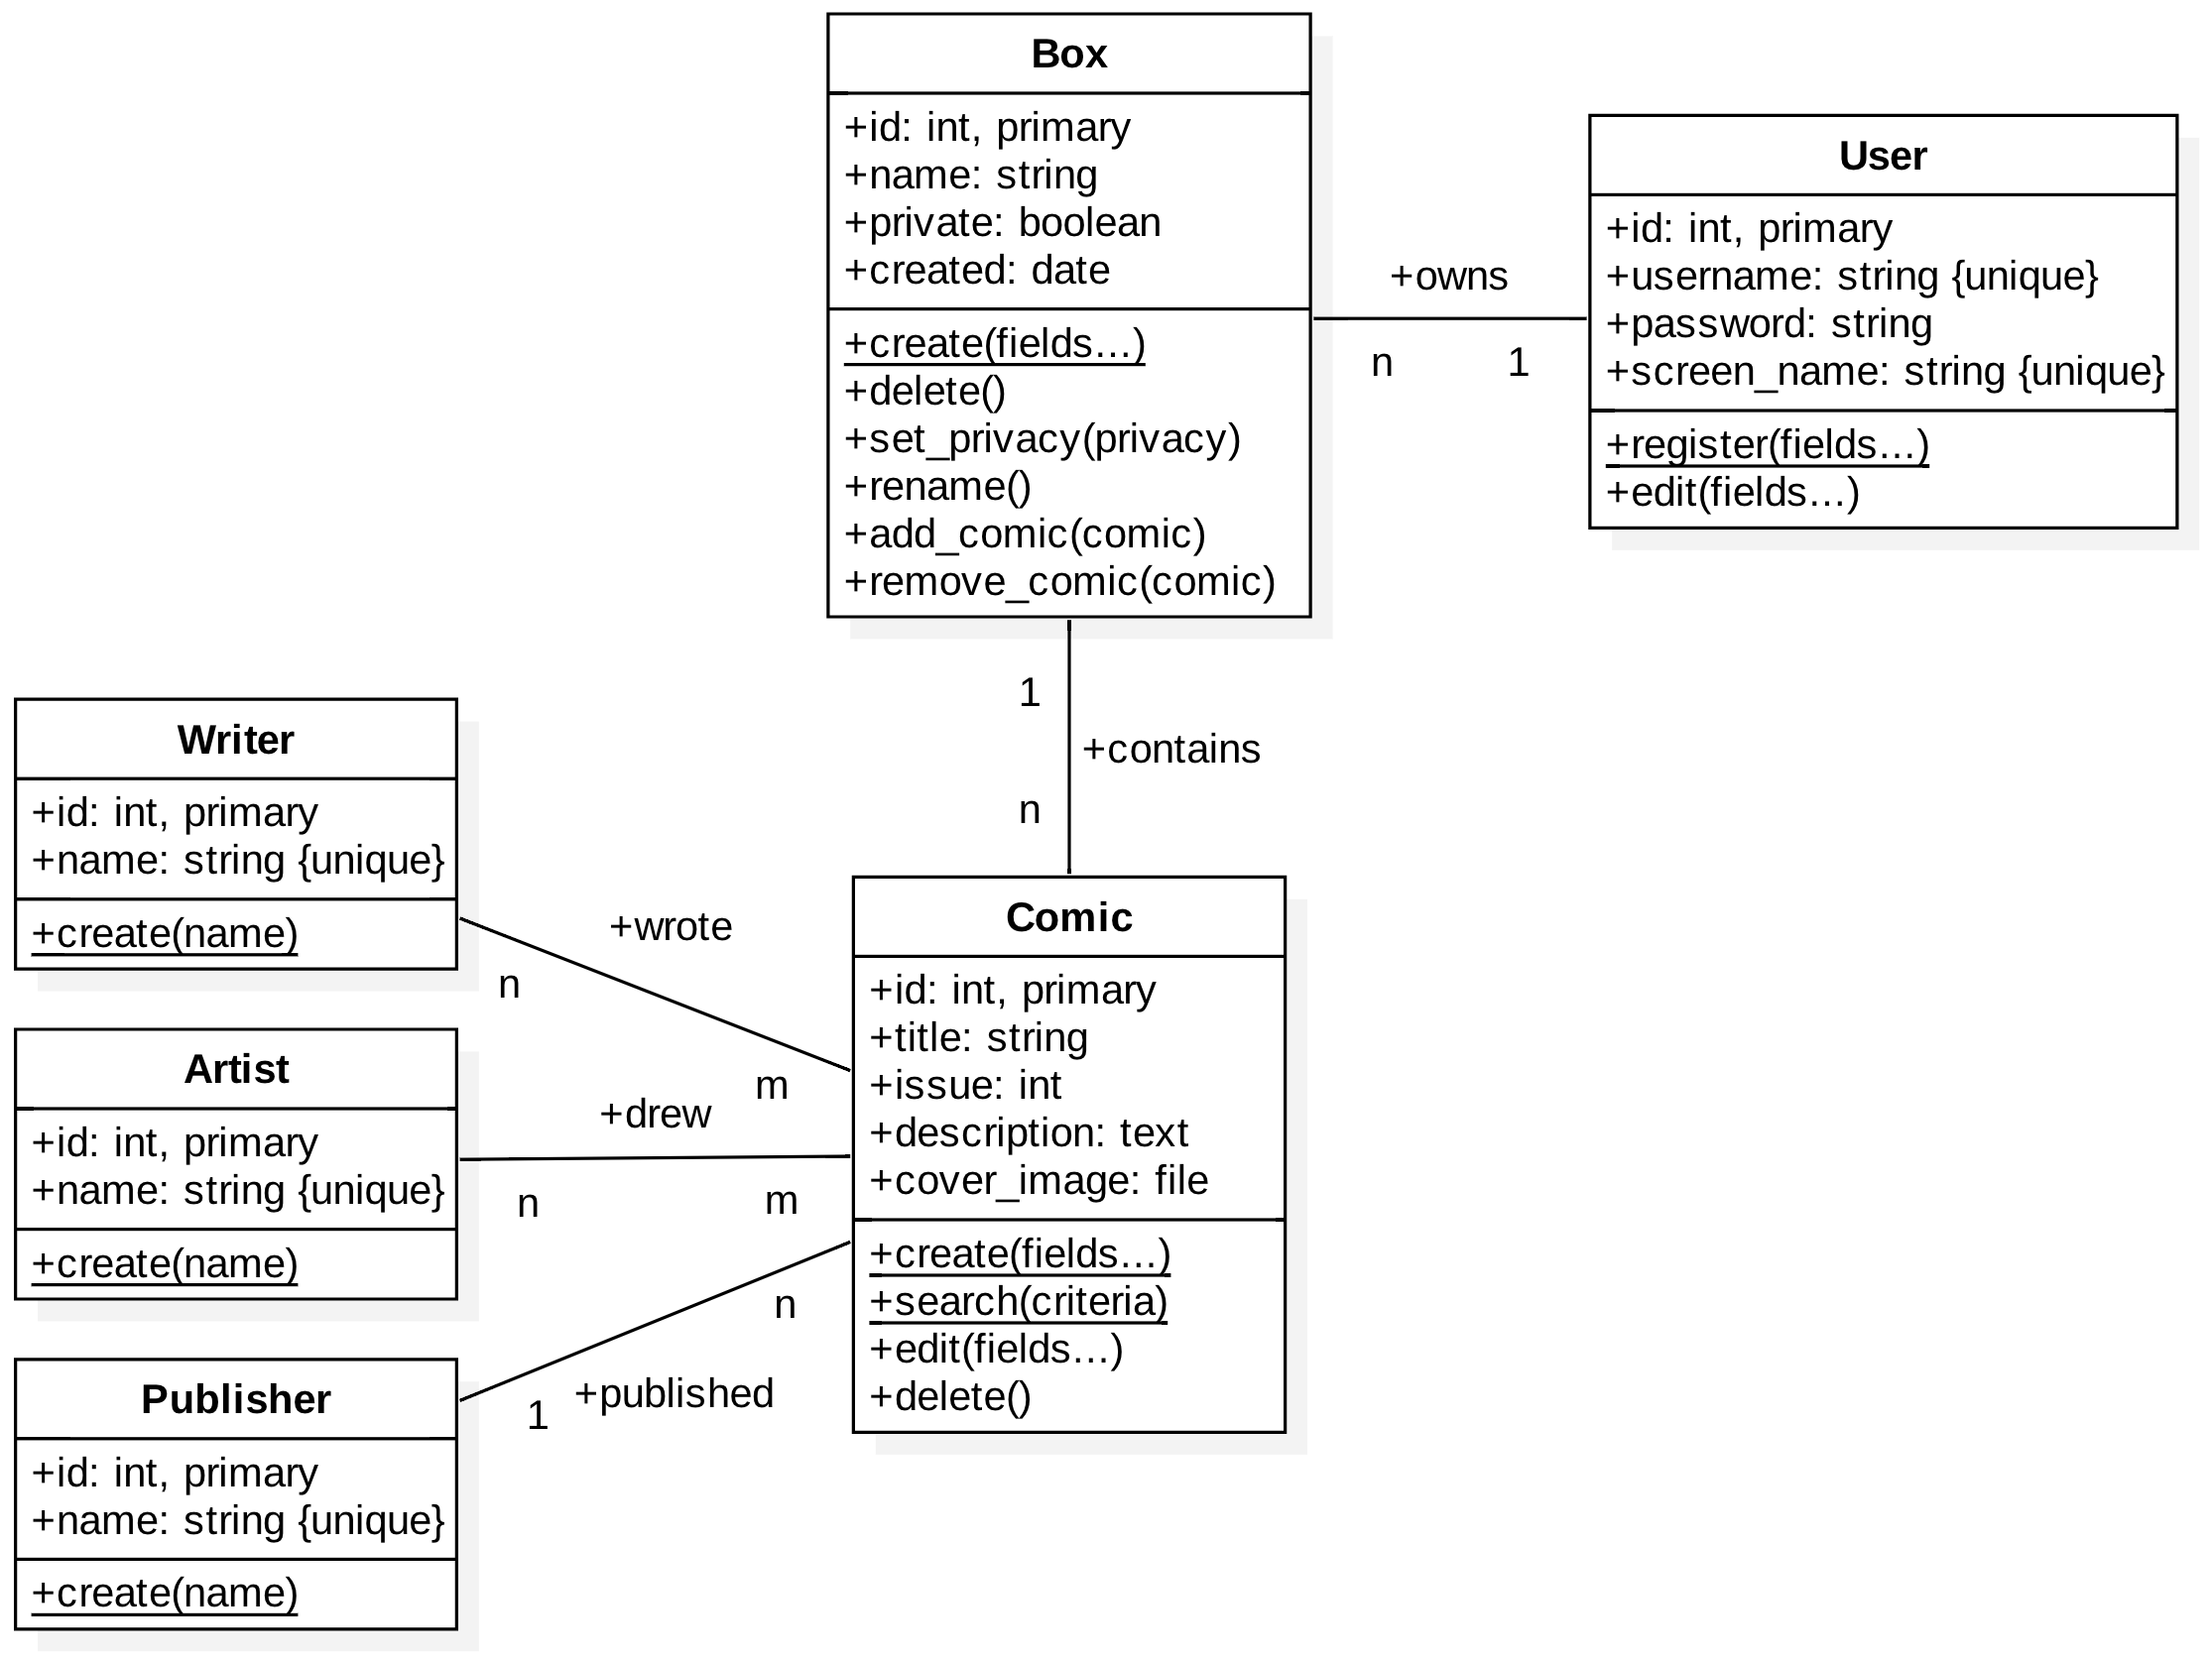
\includegraphics[width=\textwidth]{uml.png}

\subsubsection{Legend}
\begin{itemize}
  \item Primary keys are denoted by a \textsf{primary} tag after the attribute name.
  \item Underlined transactions denote that they are static, i.e., do not act upon a specific instance of the entity.
  %\item Labels on the edges between entities (relationships) should be read from \textsf{1 to n} or \textsf{n to m}. For example, \textsf{Publisher \emph{published} Comic}.
\end{itemize}

\subsubsection{Assumptions}
\begin{itemize}
  \item \textsf{Artist} and \textsf{Writer} entities were seperated from a single \textsf{Person} entity to increase extensibility and maintainability, as in the future fields specific to artists or writers may need to be added to the model.
  \item Although not noted in the diagram, \textsf{Box} names are case-insensitively unique to a \textsf{User} to prevent the potential confusion of two boxes owned by the same \textsf{User} with identical names.
  \item Integer primary keys are used in the model as they are best supported by \emph{web2py}. Alternatively, unique fields are viable candidates for being the primary key.
\end{itemize}

\section{Transaction to controller function mapping}
% [x] Demonstrate through annotation of your conceptual model that the conceptual design correctly supports the transactions needed by your application. Provide a table that maps these transactions to controller functions in the Web2Py Python controller.

\begin{tabularx}{\linewidth}{lllX}\toprule
\textbf{Model} & \textbf{Transaction} & \textbf{Controller function} & \textbf{Comments} \\ \hline

User & register & default/user/register &  \\
User & edit & default/user/profile &  \\ \hline

Box & create & box/create &  \\
Box & delete & box/delete &  \\
Box & set\_privacy & box/set\_privacy &  \\
Box & rename & box/view & \textsf{[1]} \\
Box & add\_comic & box/add\_comic &  \\
Box & remove\_comic & box/remove\_comic &  \\ \hline

Comic & create & comic/create &  \\
Comic & search & comic/search &  \\
Comic & edit & comic/edit &  \\
Comic & delete & comic/delete &  \\ \hline

\begin{tabular}[c]{@{}l@{}}Writer\\ Artist\\ Publisher\end{tabular} & \begin{tabular}[c]{@{}l@{}}create\\ delete\end{tabular} & \begin{tabular}[c]{@{}l@{}}comic/create\\ comic/edit\end{tabular} & \textsf{[2]} \\

\bottomrule
\end{tabularx}

{
  \setlength{\parindent}{0pt}
  \setlength{\parskip}{0.4em}

  \textsf{[1]} This controller function handles box renames from a form in a modal dialog on the \textsf{view} page.

  \textsf{[2]} \textsf{Writer}, \textsf{Artist} and \textsf{Publisher} entities are created on-demand as and when comics require them. When one of aforementioned entities is no longer referenced by any comic, it is deleted.
}

%-------------------------------------------------------------------------------
\chapter{Design Rationale}
%-------------------------------------------------------------------------------

% [x] Marks will be awarded for descriptions of design decisions that correctly use and reference concepts taught in class and in readings.

\begin{figure}[h!]
  \centering
  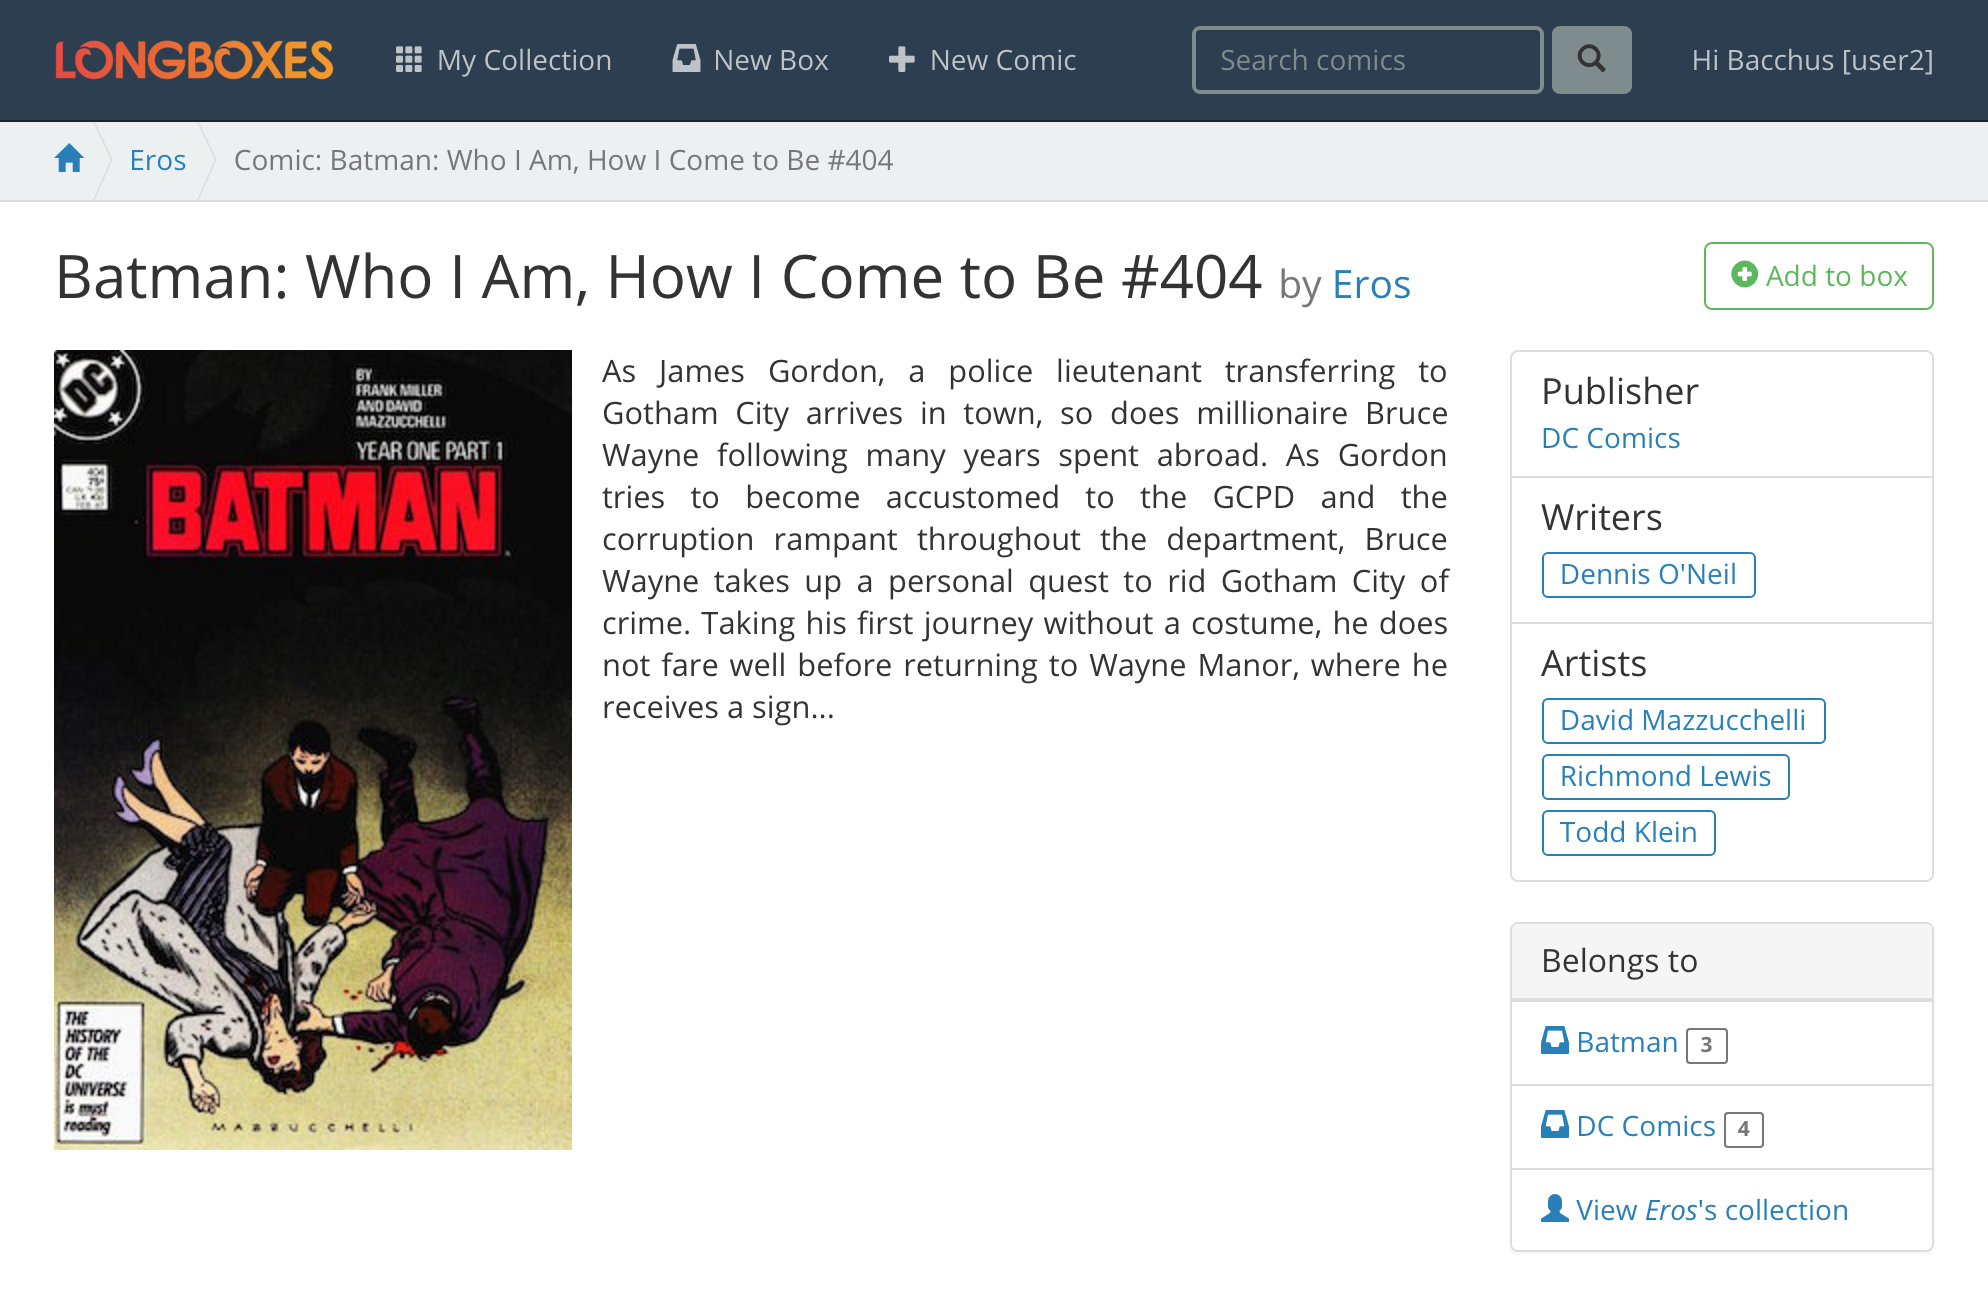
\includegraphics[width=\textwidth]{other_users_comic.png}
  \caption{
    Viewing a comic within another user's collection.
    (\texttt{/comic/view/19})
  }
  \label{fig:OtherUsersComic}
\end{figure}

\begin{figure}[b!]
  \centering
  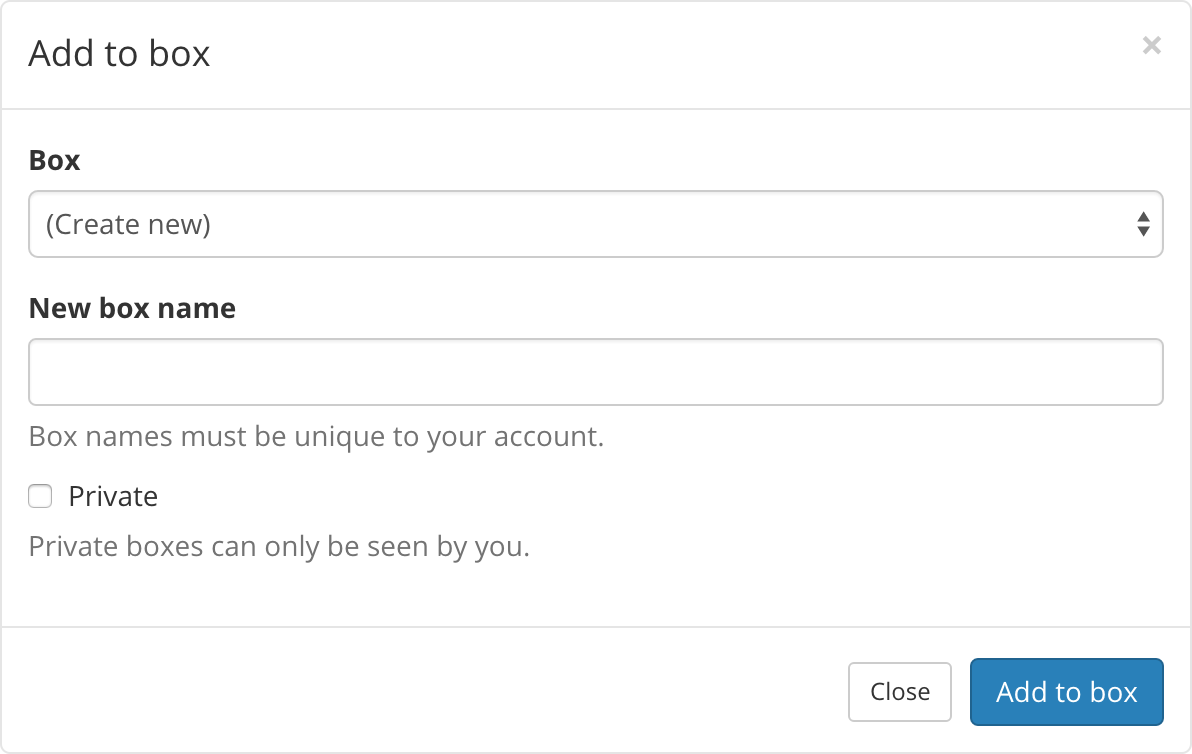
\includegraphics[width=0.7\textwidth]{add_to_box_modal.png}
  \caption{
    The modal dialog that appears when selecting \textsf{Add to box} in \autoref{fig:OtherUsersComic}.
    \textsf{Unfiled} is selected in the drop-down by default, but here \textsf{(Create new)} has been selected to demonstrate the extra fields.
  }
  \label{fig:AddToBoxModal}
\end{figure}

\newpage

\section{Supporting users through feedforward and feedback}
% Choose a user journey supported by your interface. Describe how your interface supports users through good feedforward and feedback.

% Perception
% [x] Boundaries, distinguishable features, colour
% Interpretation
% [x] Group controls, consistency
% Evaluation
% [x] Metaphors
% Intention-Action
% [x] Functional Feedforward (signposting of what actions will do)
% [x] Instructions and help
% [x] Widgets and control labelling
% Execution
% [x] Clearly indicating mandatory interaction
% [x] FEEDBACK. Need to signal to user that events have happened as a result

To demonstrate how the interface supports users through good feedforward and feedback, I will explain the interface design rationale when a user wishes to add another user's comic to their collection.

\autoref{fig:OtherUsersComic} contains several design decisions that support the user through this journey. All widgets that can be clicked (with the exception of text in the navigation bar) are coloured. For example, links in the `breadcrumb' bar, the link in the main page header, and the links on the right-side of the page all have a bright colours. In addition, the widget to add the comic to their collection (the one the user is looking for to proceed on their journey), is coloured in a green hue to stand out and to indicate that this action performs a different type of action than the others. This distinguishable green hue, and the `arrow into box' icon (used as a metaphor for placing an item into a box), is consistent with other `add comic to box' operations across the application. Note that other controls on the page are grouped logically (such as the writers, artists and containing boxes), allowing the user to gloss over groups of widgets which are not relevant to their current intention.

Upon clicking the \textsf{Add to box} button, a small modal dialog appears over the current content, as shown in \autoref{fig:AddToBoxModal}. It contains a small form with a dropdown to select the box they wish to add the comic to. At this stage the user may realise that they want to put the comic in a new box that doesn't exist yet, and by selecting the \textsf{(Create new)} option, extra fields appear at the end of the form to create a new box. This enables the user to perform the task of putting a comic in a new box without having to context switch to the \textsf{New Box} journey. The fields themselves have instructions immediately below them to explain the constraints and ramifications of that input, allowing the user to make informed decisions and reduce erroneous inputs.

The user can clearly find the button to proceed by its relatively large size and bright, filled background colour, contrasting it from the rest of the form. Through the use of the \texttt{required} attribute on the applicable \texttt{<input>} elements, the web browser prevents the form from submitting without the required fields being populated, and prompts the user in the case of an error.

Upon submitting the form, the user is redirected to the newly created comic page, and is prompted by a green banner spanning the width of the grid explaining that the transaction was successful, as shown in \autoref{fig:NewBoxFlash}. Thus completing the user journey with clear signposting and feedforward, and clear feedback on their actions whether they be valid or erroneous.

\begin{figure}[b]
  \centering
  
\includegraphics[width=\textwidth]{new_box_flash.png}
  \caption{
    Banner displayed at the top of the page after adding a comic to a new box.
  }
  \label{fig:NewBoxFlash}
\end{figure}

%-------------------------------------------------------------------------------

\newpage

\begin{figure}[p]
  \centering
  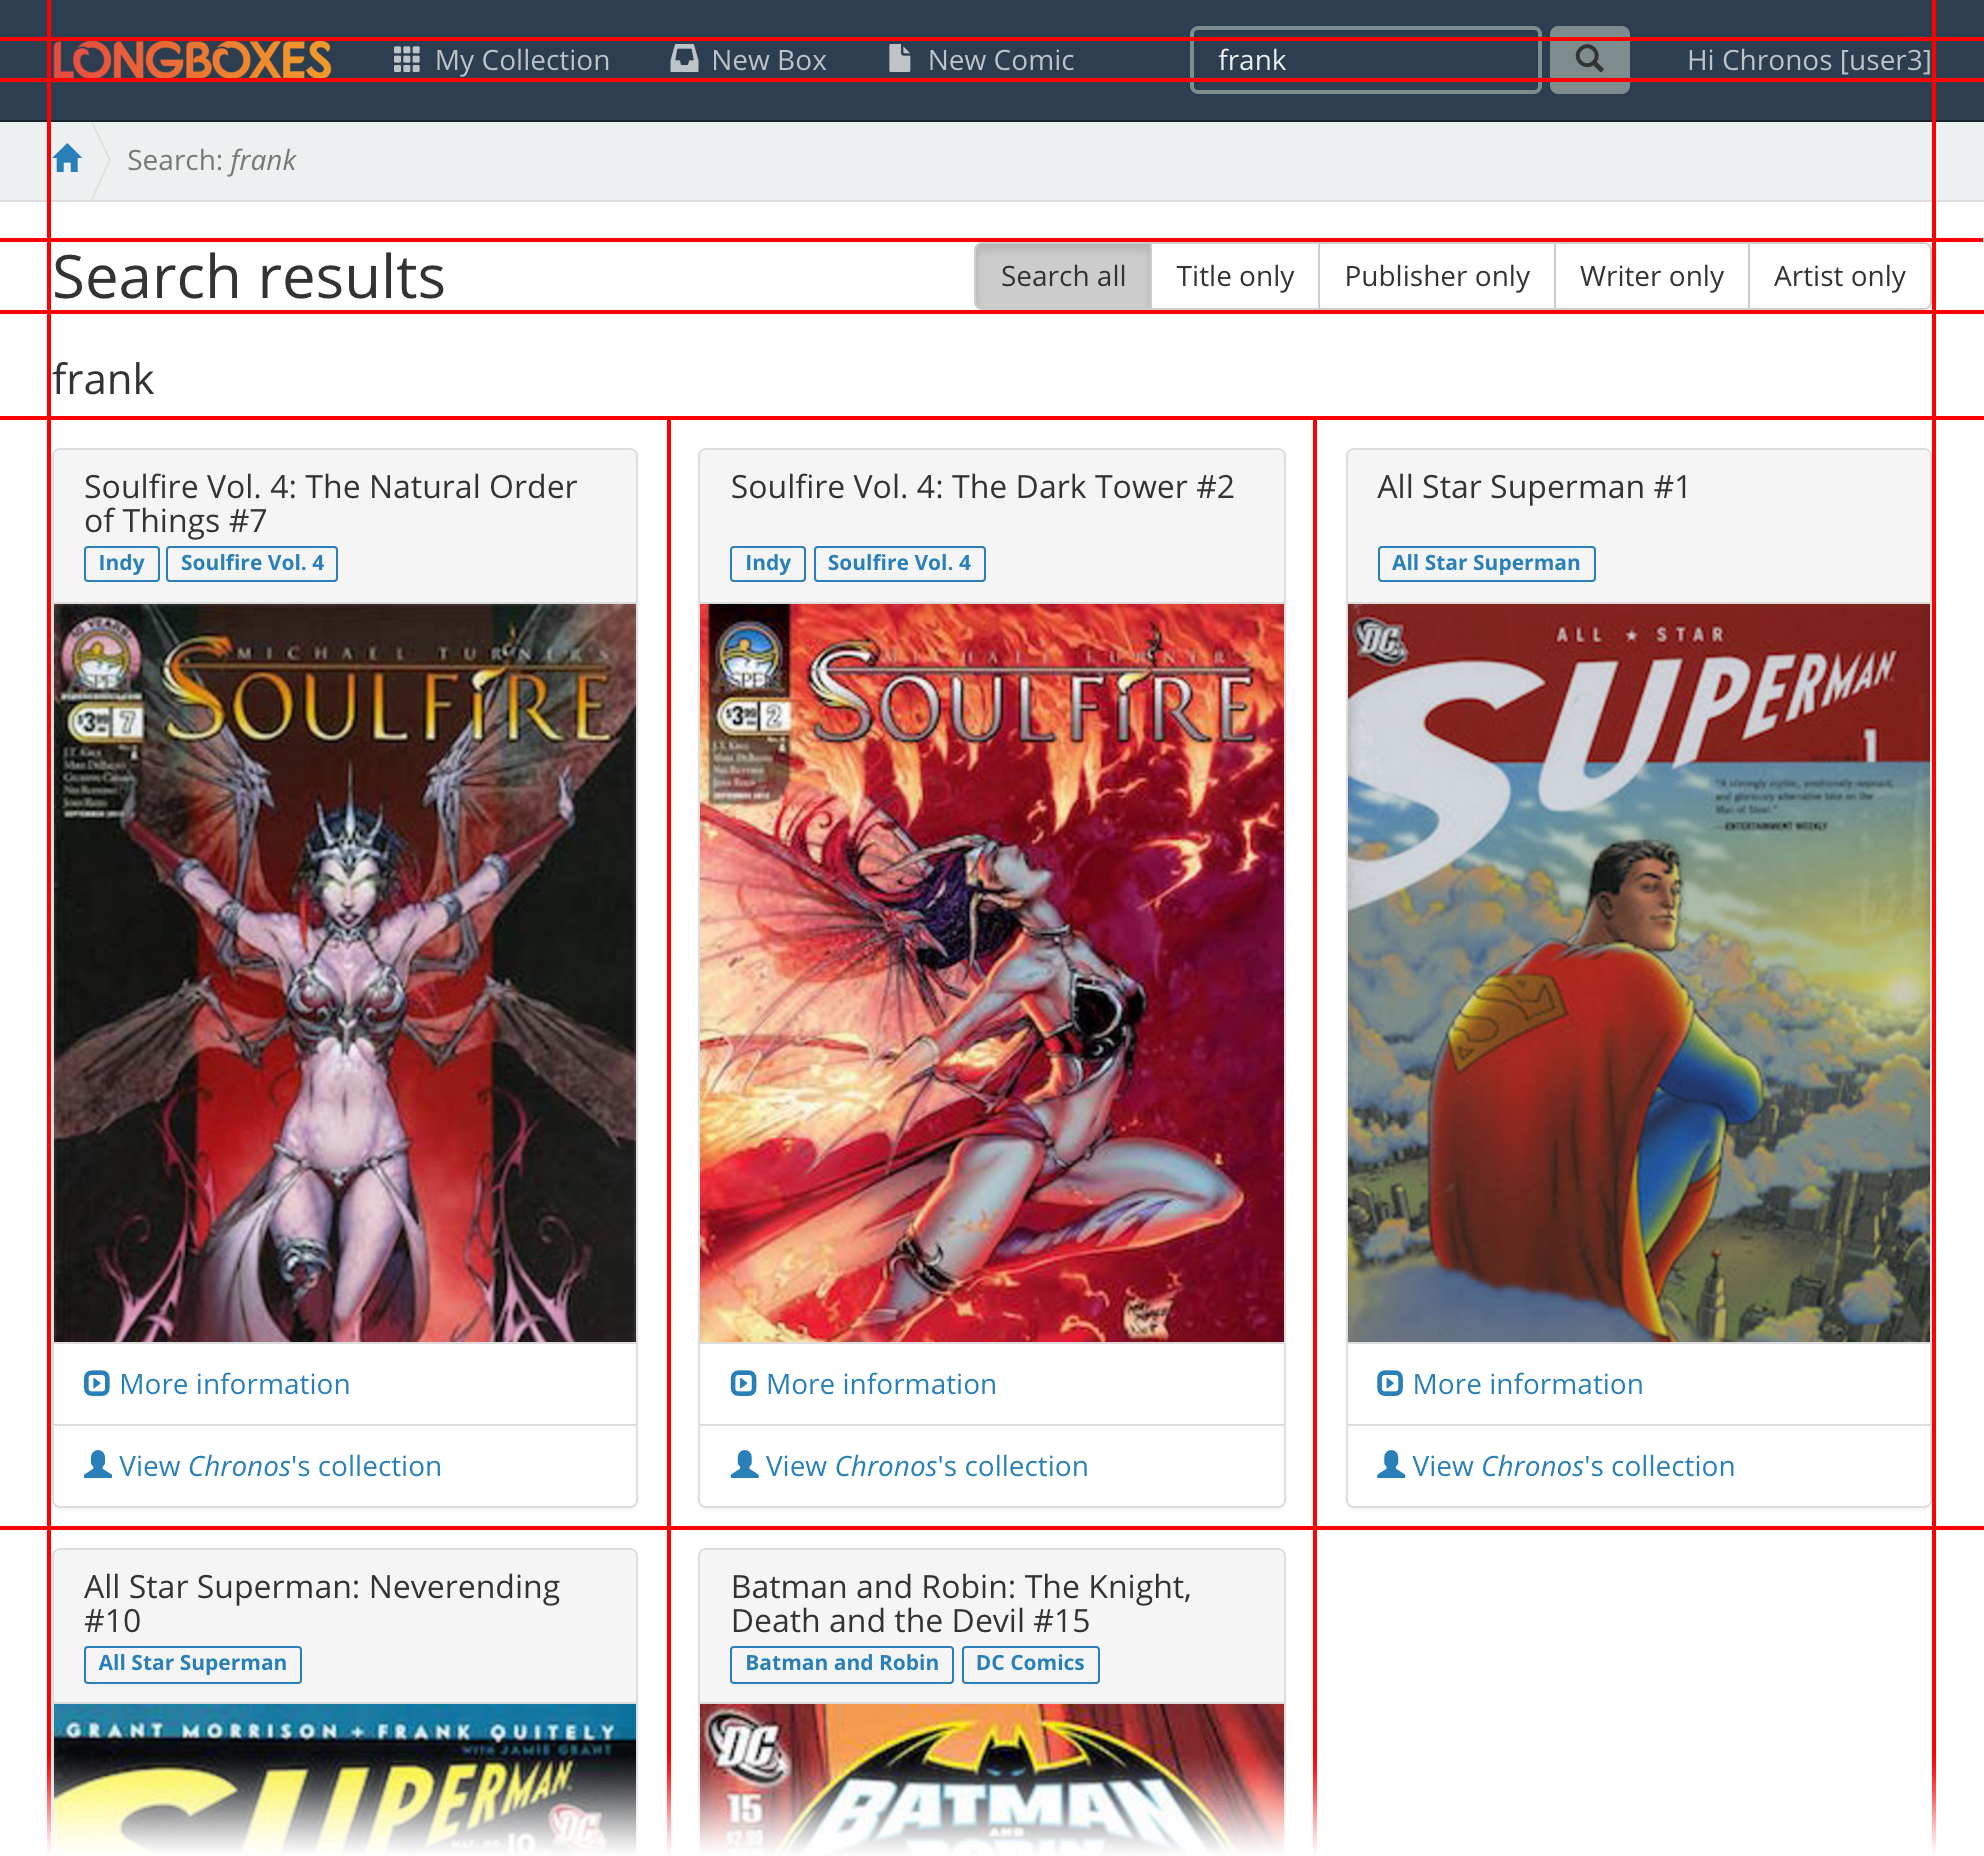
\includegraphics[width=\textwidth]{search_results.png}
  \caption{
    Search results for the \textsf{frank} query. Red lines superimposed to emphasise grid structure and the alignment of related control edges and text.
    (\texttt{/comic/search?search=frank})
  }
  \label{fig:SearchResultGrid}
\end{figure}

\begin{figure}[p]
  \centering
  
\includegraphics[width=0.5\textwidth]{comic_command_buttons.png}
  \caption{
    Command buttons on the comic detail page. \textsf{Delete} and \textsf{Edit} are only visible when the logged in user owns the comic under inspection.
  }
  \label{fig:ComicCommandButtons}
\end{figure}

\FloatBarrier

\section{Supporting users through visual layout}

% Choose a user journey supported by your interface. Describe how the visual layout supports the user in their journey.

To demonstrate how the interface supports users through visual layout, I will explain the interface design rationale when a user wishes to delete a specific comic in their collection, but cannot remember its name. For the sake of example, in this scenario the user only knows an artist of the comic and not its title.

% [x] Identify tasks that are most important to do most often - should dominate interface
% [x] Make important information prevalent
% [x] Hue, position, contrast, typography, images and size
%  - Structure
%    [x] Hierarchy, alignment of edges and margins (e.g., Grid layout)
%    [x] Grouping - through similarity and proximity
%    [x] Relationships - symbols and colours of controls

The most common tasks in the \emph{Longboxes} application have been placed in the floating navigation bar to ensure they dominate the interface. The floating position of the navigation bar ensures high visibility by always being on screen regardless of scroll position, allowing for quick access to the most common tasks. Note that apart from the logo image, no links have a high saturation in the navigation bar. This is because all of these items can be clicked, and high contrast links in this bar could distract from the main interface. However, the links' background brightens when underneath the cursor to indicate that they are interactive. The links to the left-side and centre are accompanied by icons. These icons are used across the application to refer to collections, boxes and comics to allow for immediate recognition of what a control refers to before reading the text, thereby reducing cognitive load.

For the first step in the journey, the user notes the search box in the navigation bar by its contrasting edge, muted instruction text \textsf{Search~comics} (as to not be distracting), and the magnifying glass icon, which is a ubiquitous metaphor across user interfaces to represent a search operation. The user enters the name of the artist of the comic, \textsf{frank}, and presses the \textsf{Enter} key to execute the search.

As shown in \autoref{fig:SearchResultGrid}, the comics are displayed in a grid formation below the page header. The spacing between the comic previews is consistent and spacious enough to demonstrate clear logical seperation between them. The user notices that the query returns comics of which \textsf{Frank Mastromauro} is a writer, however they are only interested in a specific comic drawn by \textsf{Frank Quitely}. As is consistent across the application, the buttons for the most common actions for that page are grouped in the top-right corner, in line with the page header. The user clicks the \textsf{Artist only} button to exclude irrelevant results.

The user finds the comic they intend to delete. To view the comic's detail page, they click the \textsf{More information} link, which has a blue hue to be consistent with other links across the application. \autoref{fig:OtherUsersComic} shows how this page looks when viewing a comic within another user's collection. In this case, as the user is viewing a comic they own, the command buttons appear as shown in \autoref{fig:ComicCommandButtons}. The user double-checks that the comic they are about to delete is in fact the correct one, which is easy due to the prevalance of important information and grouping of the comic properties on the right-side, and the large type of the comic title and owner in the page header.

The red hue of the \textsf{Delete} button distinguishes it from the other widgets, and is consistent with other destructive operations across the application. This differentiation supports the user on this journey by making it easier to find the button. Clicking the button prompts the user to confirm that they intend to irreversably delete the comic, ensuring the click was purposeful. Upon confirmation, the comic is deleted and the user is redirected to their collection with feedback notifying them that the operation completely successfully.

\end{document}
